\section{Methods} \label{section:methods}

The current implementation is a combination of two main areas of research with a motivation to accelerate Reinforcement Learning. The two areas of focus in this research will be, combining Behaviour Cloning with Reinforcement Learning which is the combination of BC + TD3 and designing an optimal reward function. This research was implemented using the deep learning framework Tensorflow \cite{tensorflow2015-whitepaper} and anaconda-python environment \cite{anaconda}. \\

\subsection{Loss Functions}

The important loss functions used for the algorithm is presented and discussed as follows. The loss functions proposed in this research is the combination of the loss functions from two similar but separate researches \cite{goecks2020integrating} \cite{nair2018overcoming}. \\

\begin{equation}\label{eq:21}
    Q_{Target} = R_t + \gamma Q(S_{t+1}, \pi(S_{t+1} | \theta_\pi ))
\end{equation}

The returns for the target Q-value used to calculate the critic loss can be written as equation \ref{eq:21}. The target Q-value is calculated for the next states and current rewards by the target actor, with or without a discount factor for future rewards determined by a terminal flag. \\

\begin{equation}\label{eq:22}
    L_{Critic} = \frac{1}{N} \sum_{i}^{N} (Q_{Target} - Q(S_{t}, \pi(S_{t} | \theta_\pi )) )^2 + L_{L2_{C}}
\end{equation}

The loss function for the critic network can be written as equation \ref{eq:22}. Both the critic networks have a similar loss function and are reduced simultaneously as the mean squared bellman error between the Q-values and target Q-values in the current sampled mini-batch. An L2 regularization loss is added to the critic values to compensate for the overfitting that might occur due to the use of demonstrations. L2 regularization \cite{cortes2012l2} has been studied and researched widely for its ability to reduce overfitting and improve generalization. Usually, L2 regularization is combined with deep learning and vision-based approaches showing great success there, but recent research on adding L2 regularization \cite{goecks2020integrating} \cite{liu2021regularization} to Reinforcement Learning models has shown to impact performance in a good way in this domain as well. \\

\begin{equation}\label{eq:23}
    L_{Actor} = -Q(S_{t}, \pi(S_{t} | \theta_\pi ))
\end{equation}

The actor loss functions aim to maximize the Q-values for the current state, the loss is calculated as the negative of the Q-values estimated by the critics which can be written as equation \ref{eq:23}. Since there are two critics predicting values to prevent the overestimation problem, the minimum of the two critic's values is taken as the final Q-value to calculate the actor loss. \\

\begin{equation}\label{eq:24}
    L_{BehaviorCloning} = \frac{1}{N} \sum_{i}^{N} [\pi(S_{t} | \theta_\pi )) - A_D ]^2
\end{equation}

The Behaviour Cloning loss is calculated as the mean squared error \cite{MSE} between the actions predicted by the agent for the states in the demonstration dataset and the actions taken by the expert demonstrator for the same states. This is a simple Behaviour Cloning loss that can be directly combined with the actor loss to train the agent. The Behaviour Cloning loss is calculated after applying the Q-filter method explained in more detail in the following section. The actor loss is maximized and the Behaviour Cloning loss is minimized. As mentioned in the previous research using this loss directly prevents the learned policy from improving significantly beyond the demonstration policy, as the actor is always tied back to the demonstrations \cite{nair2018overcoming}. \\

\begin{equation}\label{eq:25}
    L_{CombinedActor} = \lambda_{1} L_A + \lambda_{2} L_{BC} + L_{L2_{A}}
\end{equation}

The combined actor loss as shown by equation \ref{eq:25} is a direct combination of the Behaviour Cloning loss with the actor loss of the agent weighted by $\lambda$ satisfying the condition $\lambda_{2}>\lambda_{1}$. Similar to the critic loss, L2 regularization loss is added to this combined actor loss function as well. \\

\subsection{Q-Filter}

Even though the demonstrations collected are from an expert, there are many reasons for those demonstrations to be sub-optimal. To overcome this, previous research has implemented a simple strategy called Q-filter which as the name suggests filters out the demonstrations in the dataset based on the predicted Q-values which has been adopted here as well. \\

\begin{equation}\label{eq:26}
    L_{BehaviorCloning} = \frac{1}{N} \sum_{i}^{N} [\pi(S_{t} | \theta_\pi )) - A_D ]^2 || Q(S_t, A_t) > Q(S_t, \pi (S_t ))
\end{equation}

Equation \ref{eq:26} shows the Behaviour Cloning loss with Q-filter condition applied. The loss is only calculated for the states where the critic network decides that the demonstrations actions are better than the agent's actions. The states where the agent performs equal to or better than the demonstrator are not considered. The allows the agent to overcome sub-optimal demonstrations, also the agent is allowed to perform new and better actions and is not bound by the demonstrations outperforming the expert and also sometimes resulting in new behaviours. \\

\subsection{Replay Buffer}

This method uses a traditional replay buffer any other off-policy Reinforcement Learning algorithm uses without any of the advancements. But, instead of one buffer two separate buffers are introduced and maintained. First, the demo buffer of fixed length to store the demonstrations, the size depending on the number of demonstrations used. Second, the agent buffer, also of a fixed length where the agent's interactions with the environment are stored. The demo buffer has a fixed set of examples and remains stationary throughout the training process while the agent replay buffer is moving and is constantly updated on a first in first out basis as the agent continues to train and gather newer data. \\

\subsection{Demonstrations}

The number of demonstrations used varies depending on the complexity of the environment mentioned in more detail in the results section. This research focuses on two different sources of demonstrations to determine whether changing the source of demonstration has any impact on the performance of the algorithm. A very similar implementation to baseline 1 is used as an oracle \cite{AgentDemonstrations} to provide the demonstrations as the first source. This is a pre-trained model on the same environments with sparse rewards. During the sourcing of actions, 90\% of the actions were taken by the learned agent and 10\% of the actions were taken by a random agent. To the actions taken by the learned agent, Gaussian noise was added. The reason for the additional randomness and noise is to introduce sub-optimal demonstrations on purpose to simulate real-world data and also see the performance of the agent with noisy demonstrations. As these demos are sourced from an agent the success rate of the demos is the same as that of the agent, with the demos having failure examples as well. The second source of the demonstration was a handcrafted script \cite{stable-baselines} provided by the baseline team and was not developed as a part of this research. No noise was added as the script takes time to finish the task compared to the agent demonstrator with completes the task much sooner and has some time step leverage to add extra noise. Overall demonstration dataset has a mixture of both normal and noisy examples as well as successful and failure examples. \\

\subsection{Reward Design}

The reward functions for the respective environments are presented and discussed as follows. The reward functions proposed in this research are inspired and further developed from the previous research which showed good performance for a similar task \cite{nagpal2020reward}. The important fact that over-engineered reward functions can sometimes lead to sub-optimal results and also disrupt the exploration-exploitation phases of the agent was taken into consideration during the design. The main goal was to develop a simple yet informative reward function along with Behaviour Cloning to further improve the acceleration of the training of an agent. The individual components of the reward function changes based on the environment. In the equations for the reward functions D represents the distance between the respective parameters. \\

\begin{subequations}
\begin{equation}\label{eq:27a}
    R_{Reach} = -\alpha D_{Gripper-Goal}
\end{equation}   
\begin{equation}\label{eq:27b}
    R_{Reach} = +\beta \frac{1}{D_{Gripper-Goal}}
\end{equation}
\end{subequations}

The reward function for the fetch reach environment is given by equations \ref{eq:27a} and \ref{eq:27b}. When the agent is yet to reach the goal the reward is calculated as the negative distance between the gripper and the goal position in 3D space weighted by $\alpha$. This weighted negative reward motivates the agent to try and reach the goals faster. After the goal is reached by the agent a positive reward is given by taking the inverse distance between the goal and gripper weighted by $\beta$. The $\alpha$ and $\beta$ values control the strength of the negative and positive rewards respectively. This structure in design remains the same for the most part with slight variations and inclusions depending on the environment. \\

\begin{subequations}
\begin{equation}\label{eq:28a}
    R_{PickAndPlace} = -\alpha_{1} D_{Gripper-Goal} -\alpha_{2} D_{Gripper-Block} -\alpha_{3} D_{Block-Goal}
\end{equation}   
\begin{equation}\label{eq:28b}
    R_{PickAndPlace} = +\beta \frac{1}{D_{Block-Goal}}
\end{equation}
\end{subequations}

\begin{subequations}
\begin{equation}\label{eq:29a}
    R_{Push} = -\alpha_{1} D_{Gripper-Goal} -\alpha_{2} D_{Gripper-Block} -\alpha_{3} D_{Block-Goal}
\end{equation}   
\begin{equation}\label{eq:29b}
    R_{Push} = +\beta \frac{1}{D_{Block-Goal}}
\end{equation}
\end{subequations}

The reward design for the fetch pick and place and fetch push are very similar due to the dynamics of the environment. When the agent is yet to reach the goal the negative reward is calculated by the distance between the gripper and goal, the distance between the gripper and block, and the distance between the block and goal weighted by $\alpha_{1}$, $\alpha_{2}$ and $\alpha_{3}$ respectively and has to satisfy the condition $\alpha_{3}>\alpha_{2}>\alpha_{1}$. Once the agent can reach the goal the positive reward is calculated as the inverse distance between the block and the goal weighted by $\beta$. \\

\begin{subequations}
\begin{equation}\label{eq:30a}
    R_{Slide} = -\alpha D_{Block-Goal}
\end{equation}   
\begin{equation}\label{eq:30b}
    R_{Slide} = +\beta \frac{1}{D_{Block-Goal}}
\end{equation}
\end{subequations}

The reward for the fetch slide environment is calculated using only the block and goal distances without the involvement of the gripper. The reason for this is unlike the other environments which have both the desired goals and achieved goals within the space of movement of the gripper, the slide environments goals are far away from the gripper. Including the gripper distance in this reward design will confuse the agent instead of providing useful information disrupting the learning. For the fetch slide environments as shown by equations \ref{eq:30a} and \ref{eq:30b}, before the agent reaches the goal the reward is calculated as the negative distance between the block and goal weighted by $\alpha$ and after the agent reaches the goal the positive reward is calculated as the inverse of the same distance weighted by $\beta$. \\

\subsection{Training Procedure}

Before the actual training begins there is a pre-training phase that the agent goes through. After collecting the demonstrations, u a supervised learning approach the agent is pre-trained on the demonstration data even before the start of the first episode. During this pre-training phase the agent samples data from the demonstration buffer and updates its weights using the above-mentioned loss functions. This procedure shapes the initial distributions of the actor and critic networks closer to the distributions of the demonstrations which makes it easier to transition from Behaviour Cloning to Reinforcement Learning \cite{goecks2020integrating}. Additionally, before even the actual training begins this agent can perform much more meaningful actions when compared to a randomly initialized agent thus accelerating the training procedure. The Reinforcement Learning algorithm used in this research is the Twin Delayed Deep Deterministic Policy Gradient (TD3) which has shown better performance compared to its widely used predecessor DDPG. The TD3 uses simple Gaussian action noise for exploration compared to the Ornstein-Uhlenbeck \cite{Finch04ornstein-uhlenbeckprocess} uncorrelated noise. Along with the action noise 90\% of the actions are taken by the current agent and 10\% actions are taken by a random agent further aiding in exploration. During the actual training procedure, the agent is trained on 80\% of the data from the agent replay buffer and 20\% of the data from the demo replay buffer. The noise and randomness are added only during training, for testing the agent performs pure deterministic actions with the additional noise. \\

\subsection{Deep Learning Specifications}

The current algorithm uses a feed-forward neural network architecture with 3 hidden layers with 256 neurons in each layer. This is similar for both the actor and critic networks. All the hidden layers use a ELU \cite{clevert2016fast} activation function compared to the traditional RELU \cite{agarap2018deep} activation. This was motivated by previous research \cite{goecks2020integrating}, ELU has many advantages over RELU, it solves the dying RELU problem as ELU allows a certain degree of negative values while RELU cuts off to zero and is known to provide faster convergence during training. However the output layers are different, the critic network has a linear activation for estimating the Q-values while the actor-network has a TanH \cite{tanh} activation for predicting the deterministic actions. The weights of the hidden layers are initialized with He-Uniform \cite{he2015delving} initialization as this is known to work well with the RELU family of activations. The output layers are initialized with random uniform distribution for the weights, and to prevent action saturation by TanH the weights are limited to small values. L2 regularization on the weights also helps with TanH value saturation apart from controlling overfitting. Both the networks were trained with the Adam optimizer \cite{kingma2017adam}. \\

\subsection{Simulation Environments $\&$ Task Description}

\begin{figure}[h!]
    \centering
    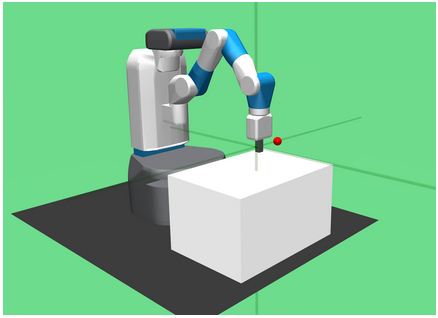
\includegraphics[width=0.8\textwidth]{images/FR.png}
    \caption{Simple Representation of the Fetch Reach Task}
    \label{fig:FR}
\end{figure}

\begin{figure}[h!]
    \centering
    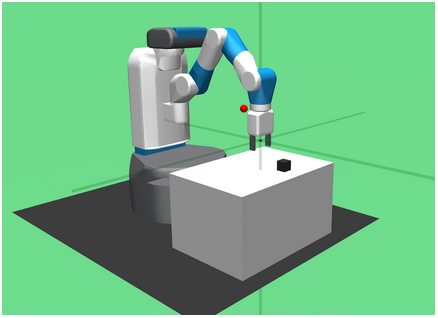
\includegraphics[width=0.8\textwidth]{images/FPAP.png}
    \caption{Simple Representation of the Fetch Pick And Place Task}
    \label{fig:FPAP}
\end{figure}

\begin{figure}[h!]
    \centering
    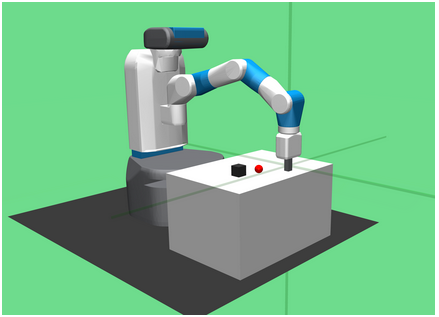
\includegraphics[width=0.8\textwidth]{images/FP.png}
    \caption{Simple Representation of the Fetch Push Task}
    \label{fig:FP}
\end{figure}

\begin{figure}[h!]
    \centering
    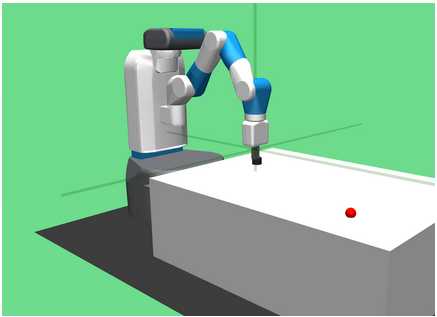
\includegraphics[width=0.8\textwidth]{images/FS.png}
    \caption{Simple Representation of the Fetch Slide Task}
    \label{fig:FS}
\end{figure}

The current implementation is tested on the Fetch Robotics Environment Suite consisting of four complex robotics interaction and manipulation tasks. The first environment is the Fetch Reach task shown in figure \ref{fig:FR}. This task is relatively simple compared to the four environments. The task here is to move the end-effector of the gripper to a randomly generated goal location. The desired goal here is the random coordinate in 3-D space and the achieved location is the position of the end-effector in the same space. The next environment is the Fetch Pick and Place Environment shown in figure \ref{fig:FPAP} where the goal is to move towards an object placed randomly on the desk, grasp it using the grippers, and move the object to the goal location either on the table or on the air. The desired goal is the position of the block and the achieved goal is the coordinate in 3-D space, both goals are randomly generated. The Fetch Push environment shown in figure \ref{fig:FP} is very similar to the previous task but with closed grippers. The task here is to use the closed grippers to push the block on the table to a goal location also on the table. It has the same desired and achieved goals as the last task and both are randomly generated anywhere on the table. The final task, also the most complex environment the suite is the Fetch Slide environment shown in figure \ref{fig:FS}. The task here is to use the closed gripper to slide a puck-like object to the goal position. It has the same desired and achieved goals as the last task and both are randomly generated anywhere on the table, with the puck spawning closer to the grippers reach and the goal spawning further down the table. \\

TODO: CHANGE IMAGES TO HIGH RES !! \\

\subsection{Algorithm Pseudocode $\&$ Hyperparameters List}

\begin{algorithm}[h!]\footnotesize
  \caption{Current Implementation Algorithm}\label{CIA}
  \begin{algorithmic}[1]
    \State Initialize Actor Network $\longrightarrow \pi(S,G | \theta_\pi )$
    \State Initialize Target Actor Network $\longrightarrow \pi^{'} (S^{'}, G | \theta_\pi^{'})$
    \State Initialize Critic 1 Network $\longrightarrow Q_{1} (S, G, A | \theta_Q )$
    \State Initialize Critic 2 Network $\longrightarrow Q_{2} (S, G, A | \theta_Q )$
    \State Initialize Target Critic 1 Network $\longrightarrow Q^{'}_{1} (S^{'}, G, A^{'} | \theta_Q^{'} )$
    \State Initialize Target Critic 2 Network $\longrightarrow Q^{'}_{2} (S^{'}, G, A^{'} | \theta_Q^{'} )$
    \State Initialize Agent Replay Buffer $M_A \longrightarrow [S, A, R, S^{'}, T] $
    \State Initialize Demo Replay Buffer $M_D \longrightarrow [S, A, R, S^{'}, T] $
    \State Load the demonstration data $\longrightarrow M_A, M_D$
    \For{Pre-Training Steps}
        \State Call PreTrainingUpdate()
    \EndFor
    \For{Episodes}
        \State Reset Env to $S_0$
        \For{Episode Timesteps}
            \If{Probability is $90\%$}
                \State Agent Takes Greedy Action $A_{t}$
            \Else{ Probability is $10\%$}
                \State Agent Takes Random Action $A_{t}$
            \EndIf
            \State Calculated Reward $R_{t}$ and Get Next State $S^{'}_{t}$ and Terminal Flag T from Env
            \State Store $[S, A, R, S^{'}, T]  \longrightarrow M_A$
            \If{Probability is $80\%$}
                \State Call TrainingUpdate()
            \Else{ Probability is $20\%$}
                \State Call PreTrainingUpdate()
            \EndIf
        \EndFor
    \EndFor
    \Procedure{PreTrainingUpdate}{}
        \State Randomly Sample Mini-Batch $[S, A, R, S^{'}, T]  \longrightarrow M_D$
        \State Calculate $L_{Critic1}, L_{Critic2}, L_{L2_{C}}$
        \State Update Critic1 and Critic2 Networks
        \If{Update Actor and Target Networks}
        \State Calculate $Q_1 \& Q_2 \longrightarrow Critic_1 \& Critic_2$, $\min(Q_1, Q_2)$
        \State Calculate $Q_{min}, L_{Actor}, L_{BC}, L_{L2_{A}}, L_{CombinedActor}$
        \State Update Actor Network
        \State Update Target Actor Networks
        \Else{}
            \State Continue
        \EndIf
    \EndProcedure
    \Procedure{TrainingUpdate}{}
        \State Randomly Sample Mini-Batch*0.90 $[S, A, R, S^{'}, T]  \longrightarrow M_A$
        \State Randomly Sample Mini-Batch*0.10 $[S, A, R, S^{'}, T]  \longrightarrow M_D$
        \State Calculate $L_{Critic1}, L_{Critic2}, L_{L2_{C}}$
        \State Update Critic1 and Critic2 Networks
        \If{Update Actor and Target Networks}
        \State Calculate $Q_1 \& Q_2 \longrightarrow Critic_1 \& Critic_2$, $\min(Q_1, Q_2)$
        \State Calculate $Q_{min}, L_{Actor}, L_{BC}, L_{L2_{A}},  L_{CombinedActor}$
        \State Update Actor Network
        \State Update Target Actor Networks
        \Else{}
            \State Continue
        \EndIf
    \EndProcedure
  \end{algorithmic}
\end{algorithm}

\begin{table}[h!]
\centering
\begin{tabular}{|c|c|}
\hline
\textbf{Hyperparameters}                       & \textbf{Values}                          \\ \hline
Agent Replay Memory Size              & 1000000                         \\ \hline
Reach Demo Memory Size                & 20*50                           \\ \hline
Pick and Place Demo Memory Size       & 40*50                           \\ \hline
Push Demo Memory Size                 & 40*50                           \\ \hline
Slide Demo Memory Size                & 40*50                           \\ \hline
Critic Network Size                   & 256 x 256 x 256                 \\ \hline
Actor Network Size                    & 256 x 256 x 256                 \\ \hline
Optimizer                             & Adam                            \\ \hline
Optimizer Learning Rate               & 0.001                           \\ \hline
Weight Initialization Hidden Layer    & he\_uniform                     \\ \hline
Weight Initialization Output Layer    & random\_uniform (-0.003, 0.003) \\ \hline
Hidden Layer Activations              & ELU                             \\ \hline
Critic Output Activation              & Linear                          \\ \hline
Actor Output Activation               & TanH                            \\ \hline
L2 Regularization                     & 0.01                            \\ \hline
Gaussian Noise                        & Mean: 0, Std: 0.1               \\ \hline
Actor and Target Networks Update Step & 2                               \\ \hline
Agent Mini Batch                      & 1024                            \\ \hline
Demo Mini Batch                       & 128                             \\ \hline
Target Actions Noise                  & Mean: 0, Std: 0.2               \\ \hline
Target Actions Clip Range             & (-50, 0.5)                      \\ \hline
Discount Rate                         & 0.98                            \\ \hline
Combined Loss Lambda1                 & 1.0                             \\ \hline
Combined Loss Lambda2                 & 2.0                             \\ \hline
Positive Reward Beta                  & 0.01                            \\ \hline
Negative Reward Alpha                 & 5.0                             \\ \hline
Negative Reward Alpha1                & 1.0                             \\ \hline
Negative Reward Alpha2                & 2.0                             \\ \hline
Negative Reward Alpha3                & 3.0                             \\ \hline
\end{tabular}
\caption{Detailed List of Hyperparameters Used.}
\label{tab:my-table}
\end{table}
